This chapter focuses on a precise estimate of the search background. The
background prediction is of crucial importance for searches beyond the SM because an observation
of an upward deviation with respect to the background prediction may hint at a new discovery.
First, a data-driven background estimate is introduced. The benefit of a data-driven technique
as compared to a simulation-based estimate is that it avoids possible issues of 
mismodelling. Finally, tests of the background estimate are performed 
in control regions to establish the correctness of the method and to assess
its systematic uncertainty.


\section{Method of uncorrelated variables (ABCD)}


% We use an extension of the ABCD method 
% a little paragraph in there saying something like: to establish the notation, we consider a simple version of the ABCD method
% involving two independent cuts. 

% make an introduction about the ABCD method for only two variables

\label{sec:abcd}
We use a data-driven method of independent selections, ``the ABCD method".
To establish the notation, we introduce a simple version of the method that involves two 
independent selection criteria. As schematically presented in Fig.~\ref{fig:abcd} 
with two selection criteria one can divide the events into four
regions.
\begin{figure}[htbp]
\centering
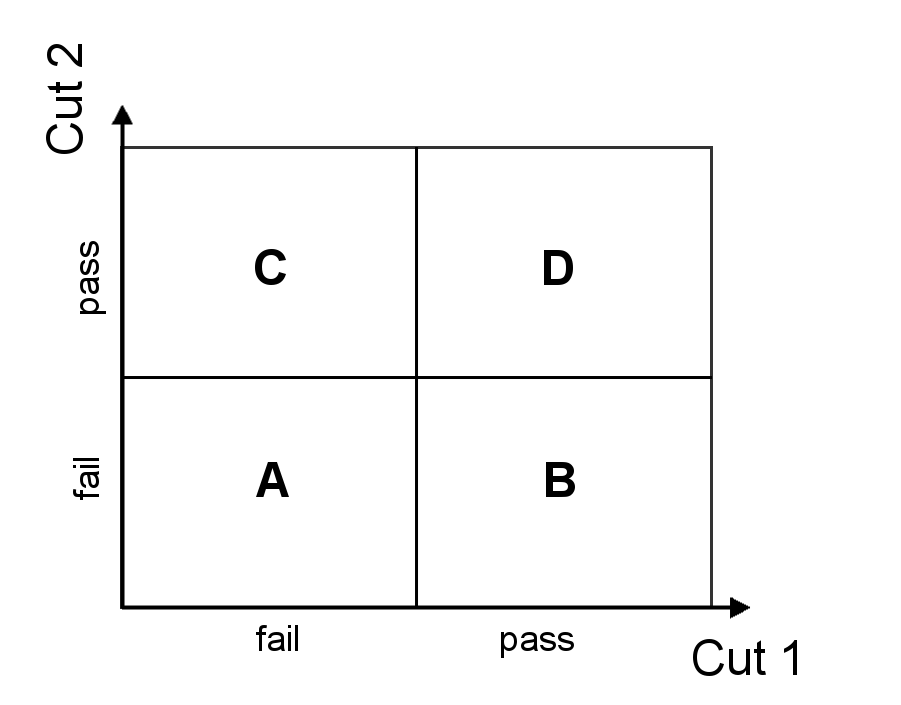
\includegraphics[width=0.65\textwidth]{plots/abcd.png}
\caption{Naming convention for the regions used in ``the ABCD method".\label{fig:abcd}}
\end{figure}
The regions A, B, and C are background dominated because the events that fall into those regions fail at least 
one of the selection criteria which have been optimized for signal detection. 
Given that for background events the probability of passing the first criterion is independent 
from whether it passes the second criterion, the number
of background events in the signal region, D, can be obtained from the event counts in regions A, B and C using the formula:

\begin{equation}
\text{D} = \frac {\text{BC}}{\text{A}}
\end{equation}


In this analysis, we use an extension of ``the ABCD method" using
 three, instead of two, independent selection criteria, see Section \ref{sec:selection} for the definitions of those criteria for displaced dijets. 
The three selection criteria divide the events into eight
regions (A, B, C, ..., H), as listed in Table \ref{tab:regions}, with  H being the signal region.

\begin{table}[htbp]
\centering
\caption{Naming convention for the regions used in background estimation. "+" corresponds to a selection 
being applied, while "--" to a selection being inverted. \label{tab:regions}}
\vspace{0.1cm}
\begin{tabular}{cccc}
 \hline
  Region & selection 1 & selection 2 & selection 3 \\
 \hline
 A & -- & -- & -- \\
 B & + & -- & -- \\
 C & -- & + & -- \\
 D & -- & -- & + \\
 E & -- & + & + \\
 F & + & -- & + \\
 G & + & + & -- \\
 H & + & + & + \\
\hline
\end{tabular} 
\end{table}

With three independent selections the background level in the signal region H can be estimated from various combinations
of the event counts in other regions. Among the suitable combinations 
there are six that use event counts in only
three regions, namely:
\begin{enumerate}
 \item FG/B = (+,--,+)(+,+,--) / (+,--,--) -- the right hand side of the equation uses
 a notation that indicates which selections are passed and which are failed by 
 the events in a given region
 \ie (+,--,+) corresponds to region F where events pass the first and third selection,
 while they fail the second selection;
 \item EG/C = (--,+,+)(+,+,--) / (--,+,--)
 \item EF/D = (--,+,+)(+,--,+) / (--,--,+)
 \item DG/A = (--,--,+)(+,+,--) / (--,--,--)
 \item BE/A = (+,--,--)(--,+,+) / (--,--,--)
 \item CF/A = (--,+,--)(+,--,+) / (--,--,--)
\end{enumerate}


%\begin{itemize}
%\item FG/B, EG/C, EF/D - for these background estimates the numerator regions are such that two selections
%are applied and one is inverted, while the denominators are regions where one selection
%is applied and two are inverted;
%\item DG/A, BE/A, CF/A - the numerators are such that the two regions taken together involve
%all three selections both applied and inverted

%for these background estimates two selections are combined into one
%and therefore we apply and inverted
%these choices combine two selections together and apply or invert it with the 
%remaining selection.
%\end{itemize}

A seventh background prediction can be formed by combining three of the predictions above:

\begin{equation}
\frac{\text{DG/A}\cdot\text{BE/A}}{\text{EG/C}} = \frac{\text{BCD}}{\text{A}^2} = \frac{(+,-,-)(-,+,-)(-,-,+)}{(-,-,-)^2}
\end{equation}


The combination BCD/A$^2$ is constructed from regions with at least two selections inverted.
It minimizes the statistical uncertainty on the background estimate, because in regions 
A, B, C, and D
the background event counts are largest. We use BCD/A$^2$ as our background prediction
central value.
%A seventh background prediction, which minimizes statistical uncertainty,
%can be formed by combining three of the estimates above:
%\begin{equation}
%DG/A * BE/A / EG/C = BCD/A^2
%\end{equation}
In the case of perfectly independent 
variables, all of the combinations above predict statistically consistent  amounts of background. 
However, to account for possible systematic
effects due to residual dependence of the selections, we assign a systematic uncertainty 
that is equal to the largest difference 
between BCD/A$^2$ and any of the six other predictions.

\section{Selection optimisation}
\label{sec:cutvalues}
We determine the numerical values of the selection criteria that are employed in the background estimation procedure 
by optimizing the expected limit for each tested signal model.
The signal models considered include various values of the \Higgs mass, the \X mass, and the \X lifetime.
The selection variables
do not strongly depend on the particles masses, therefore the optimal selection criteria
vary only as a function of the
mean transverse decay length ($L_{xy}$)
of the \X bosons. We use two sets of selection criteria,
depending on whether the mean
$L_{xy}$ of the \X bosons is below or above 30\cm. The selection criteria are
detailed in Table \ref{tab:background}.

\begin{table}[htbp]
\centering
\caption{Optimised selection criteria and the corresponding background expectations with their statistical and systematic uncertainties.\label{tab:background}}
\vspace{0.1cm}
\begin{tabular}{r|c|c}
%\hline
$\bf L_{xy}$ \bf selection &\bf  $\bf <30\cm (low)$ & \bf  $\bf >30\cm (high)$ \\
\hline
prompt tracks & $\leq1$ & $\leq1$ \\
%\hline
prompt energy & $<0.15\%$ & $<0.09\%$ \\
%\hline
vertex/cluster disc. & $>0.9$ & $>0.8$  \\
\hline
\bf expected bkg. & $\bf 1.60\pm0.26(stat)\pm0.51(syst)$ & $\bf 1.14\pm0.15(stat)\pm0.52(syst)$ \\
%\hline
\end{tabular}
\end{table}

\section{Background tests}
\label{sec:backgroundtests}
The background estimation procedure described in Section \ref{sec:abcd} is general and can be applied
to any dataset if the selections used are independent.
In this section we describe various background closure tests
 performed in QCD MC simulation and 
selected control regions in data.
We test the optimal selection criteria from Section \ref{sec:cutvalues} and also other various selections points.
%In order to perform background tests we apply various selections, not only the optimal ones
%listed in Section \ref{sec:cutvalues}.
The figures shown in the following sections present the observed number
of events along with the seven background estimates which were described
 in Section \ref{sec:abcd}.
Uncertainties are statistical only. 
For each of the tested selection points the background prediction 
and its uncertainty are obtained 
using the prescription from Section \ref{sec:abcd}. 
%The background prediction and its statistical 
%and systematic uncertainties are
% not explicitly plotted given that all of the 7 combinations employed in its derivation are shown.  
The compatibility between the predicted and observed background is estimated with a {\it p-value} for each measurement. 
%The {\it p-values} are then converted into {\it significances} using the normal distribution. 
 The {\it p-value}
is computed with respect to the estimated background probability density function (p.d.f.). 
The background prediction has an associated uncertainty, 
therefore the background p.d.f. is a Poissonian function convolved  
with a Gaussian error function. The probability of observing $n$ background events is given by:
\begin{equation}
B(n,b,\sigma_b)= \frac{1}{\sqrt{2\pi}\sigma_b} \int_{0}^{\infty} 
\exp\left[ -\frac{\left(x-b\right)^2}{2\sigma_b^2}\right]\frac{x^n e^{-x}}{n!}dx
\label{eqn:bdensity}
\end{equation}
where $b$ is the background central value and $\sigma_b$ is the total uncertainty.
The Gaussian probability density of the background mean has been truncated at 
0 in order to avoid unphysical values. Such a truncation results in a not properly normalized p.d.f. in Eq. 
\ref{eqn:bdensity}, however the {\it p-values} computed according to Eq. \ref{eqn:pvalues} take the 
normalization into account.   
\begin{equation}
{\it p} (n_\text{obs},b,\sigma_b) = \sum_{k\geq n_{obs}} B(k,b,\sigma_b) / \sum_{k} B(k,b,\sigma_b)
\label{eqn:pvalues}
\end{equation}
The {\it p-values} are then converted into {\it significances} using the normal
 distribution. The {\it significances} are shown in the bottom plots (Figs. 
\ref{fig:bkg_MC}-\ref{fig:10percent}) aligned to the corresponding background
measurements.  

\subsection{QCD MC background prediction}
\label{subsec:bkgQCDMC}

Due to the limited statistics of the QCD MC samples, the displaced jet trigger requirement has been removed. In addition, the background is estimated with looser
 selection on prompt tracks variables compared to the final selection. 
In order to validate the background prediction with 
the observed Poissonian event counts, the cross-section weights (Table \ref{tab:backgrMC}) 
are removed. 
Therefore this test serves only to identify biases due to non-independent selections,
and cannot be translated
into a background prediction in data.  
As shown in Fig. \ref{fig:bkg_MC} good agreement between predicted and observed background level is found, 
and the discrepancy is not significant for the tested selection points. Therefore, we conclude that the  
bias due to possible interdependence between the variables is small in the QCD MC samples. 

\begin{figure}[htbp]
  \centering
  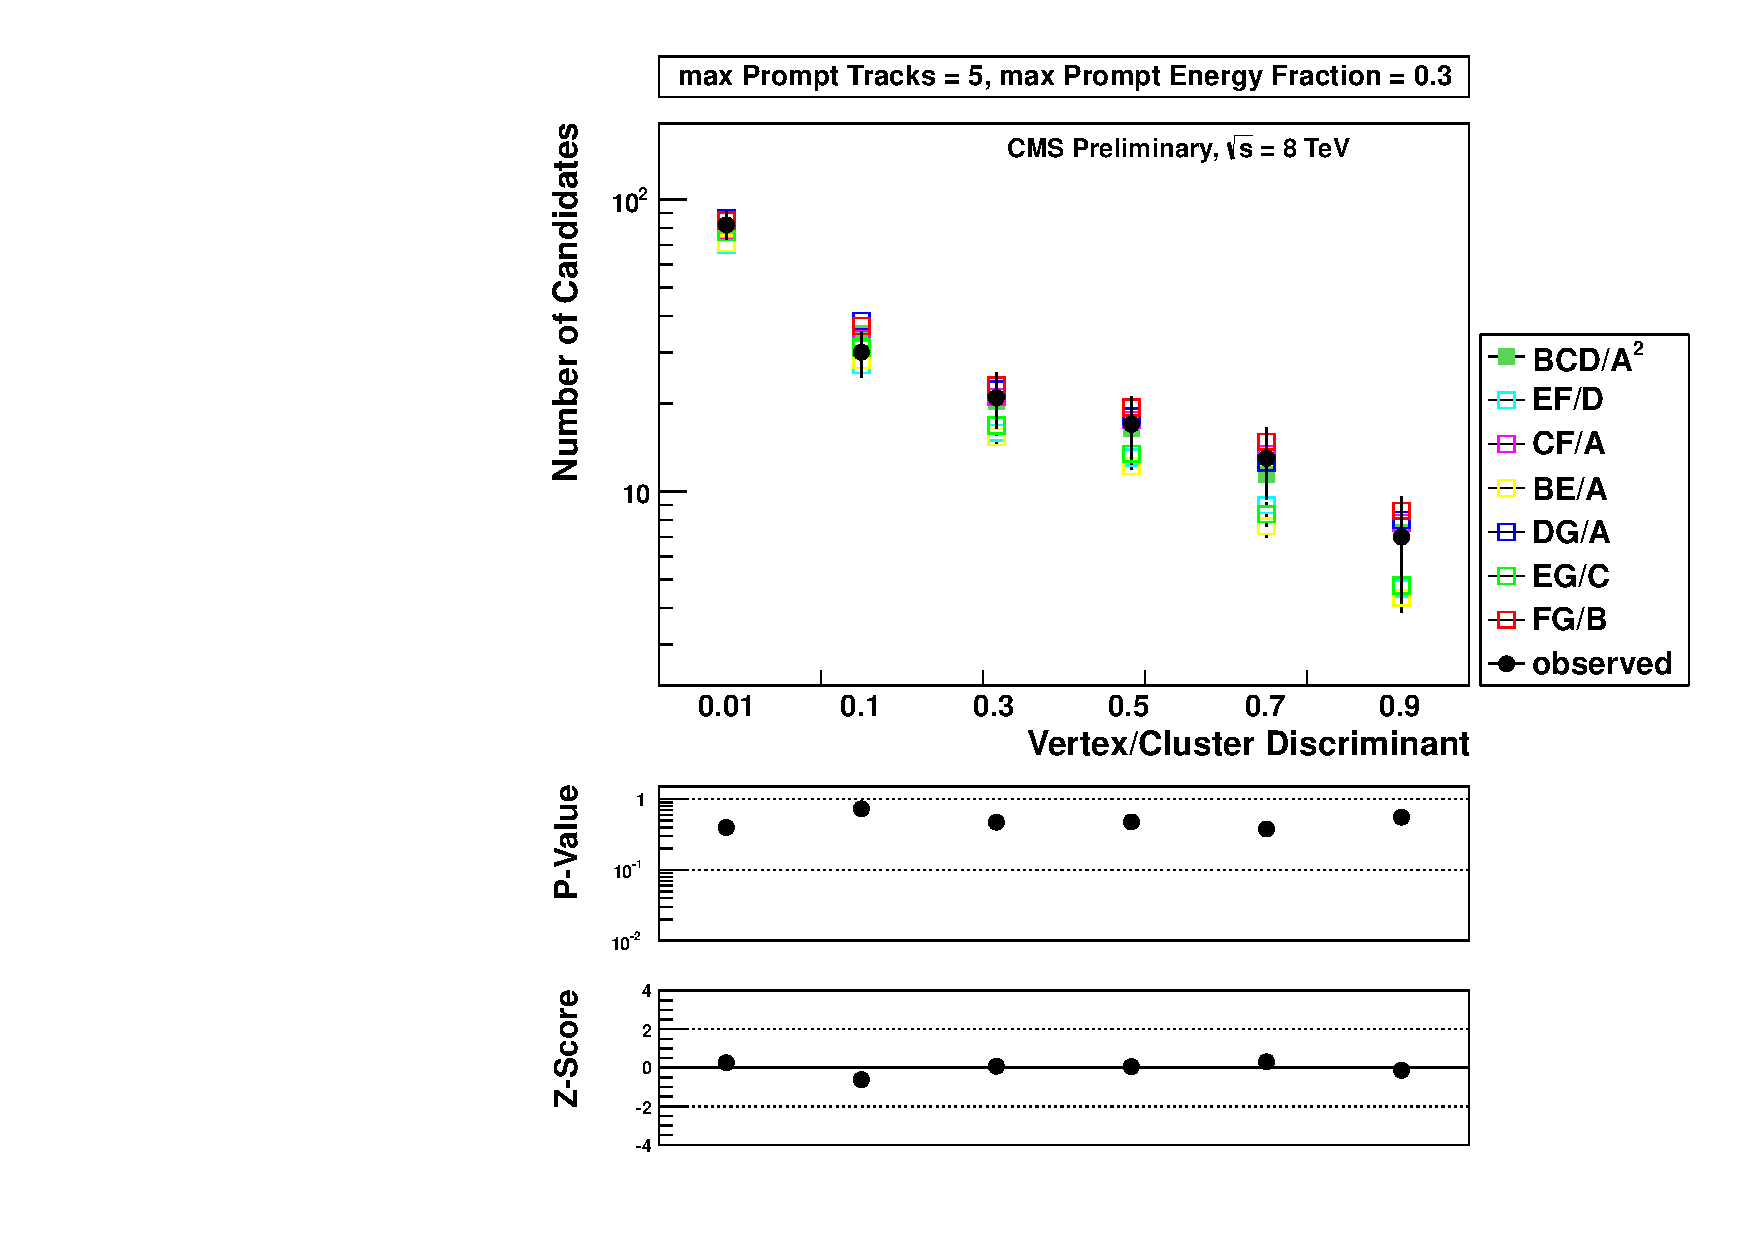
\includegraphics[width=0.495\textwidth]{plots/background/bkg_MC1.pdf}
  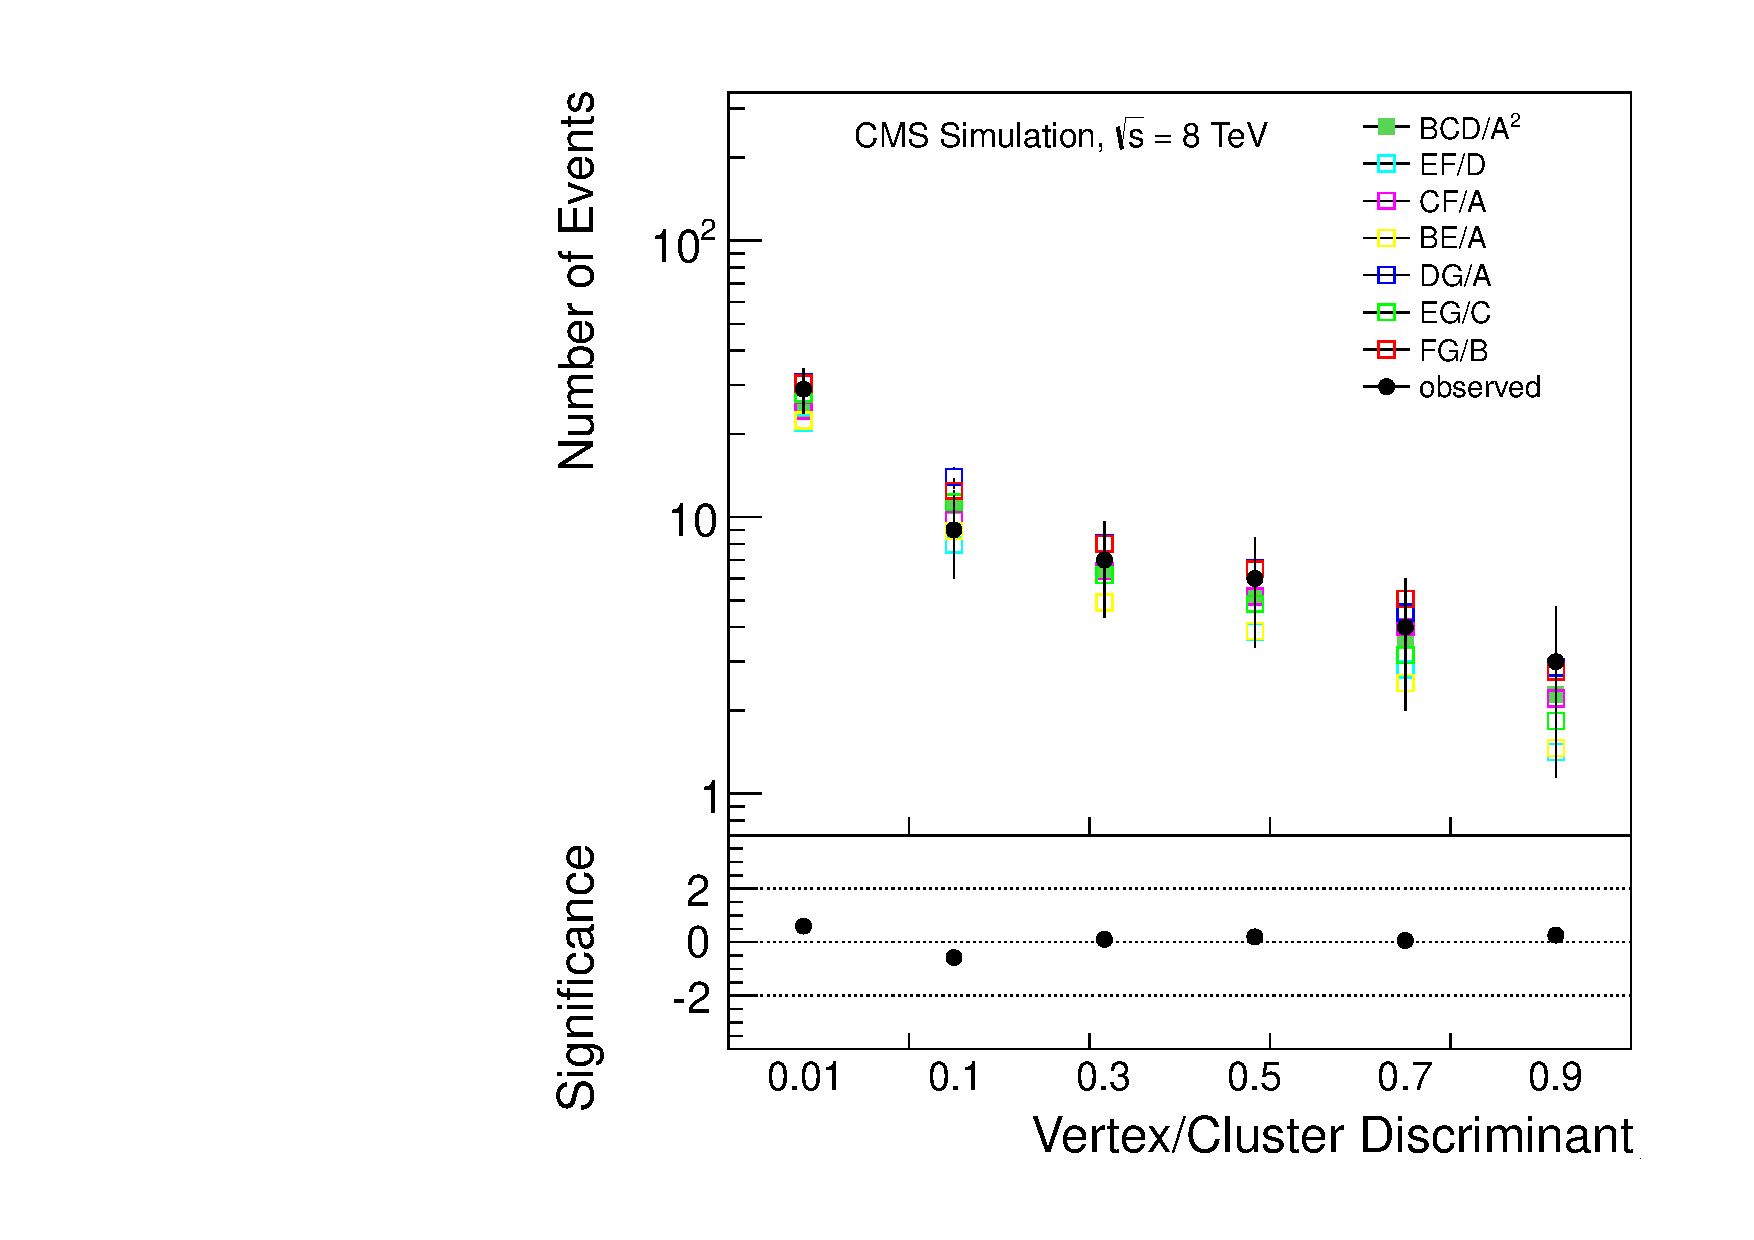
\includegraphics[width=0.495\textwidth]{plots/background/bkg_MC2.pdf}
  \caption{Predicted and observed background levels for the QCD MC sample as a function of the vertex discriminant selection criteria.
The selection requires at most 5 (left) and 4 (right)  prompt tracks and that their jet energy fraction be below 30\% (left) and 25\% (right), which
is significantly looser than the final selection. \label{fig:bkg_MC}}
  \end{figure}


\subsection{Data control region}
\label{subsec:bkgCtrl}

As a data control region we use candidates passing all of the preselection criteria listed in Section
 \ref{sec:selection}, but with the {\it missing hits} selection inverted. We again choose only 
 one candidate per event, applying the same procedure as described in Section \ref{sec:selection}.
 Such a region has a very small 
signal acceptance compared to the signal region, as the {\it missing hits} criterion has a very high signal 
efficiency, while providing a
background sample with good statistics. Using this control region we are able to test final selection
criteria with amounts and uncertainties of predicted background comparable to the signal region. 
 As shown in Fig. \ref{fig:bkg_NMiss}, 
the background predictions in this control region are in good agreement 
with the observed background levels. Given that the significance
of the discrepancies is small, we conclude
that the background estimation method is valid and the systematic uncertainty on the background
 prediction is not underestimated.

\begin{figure}[htbp]
\centering
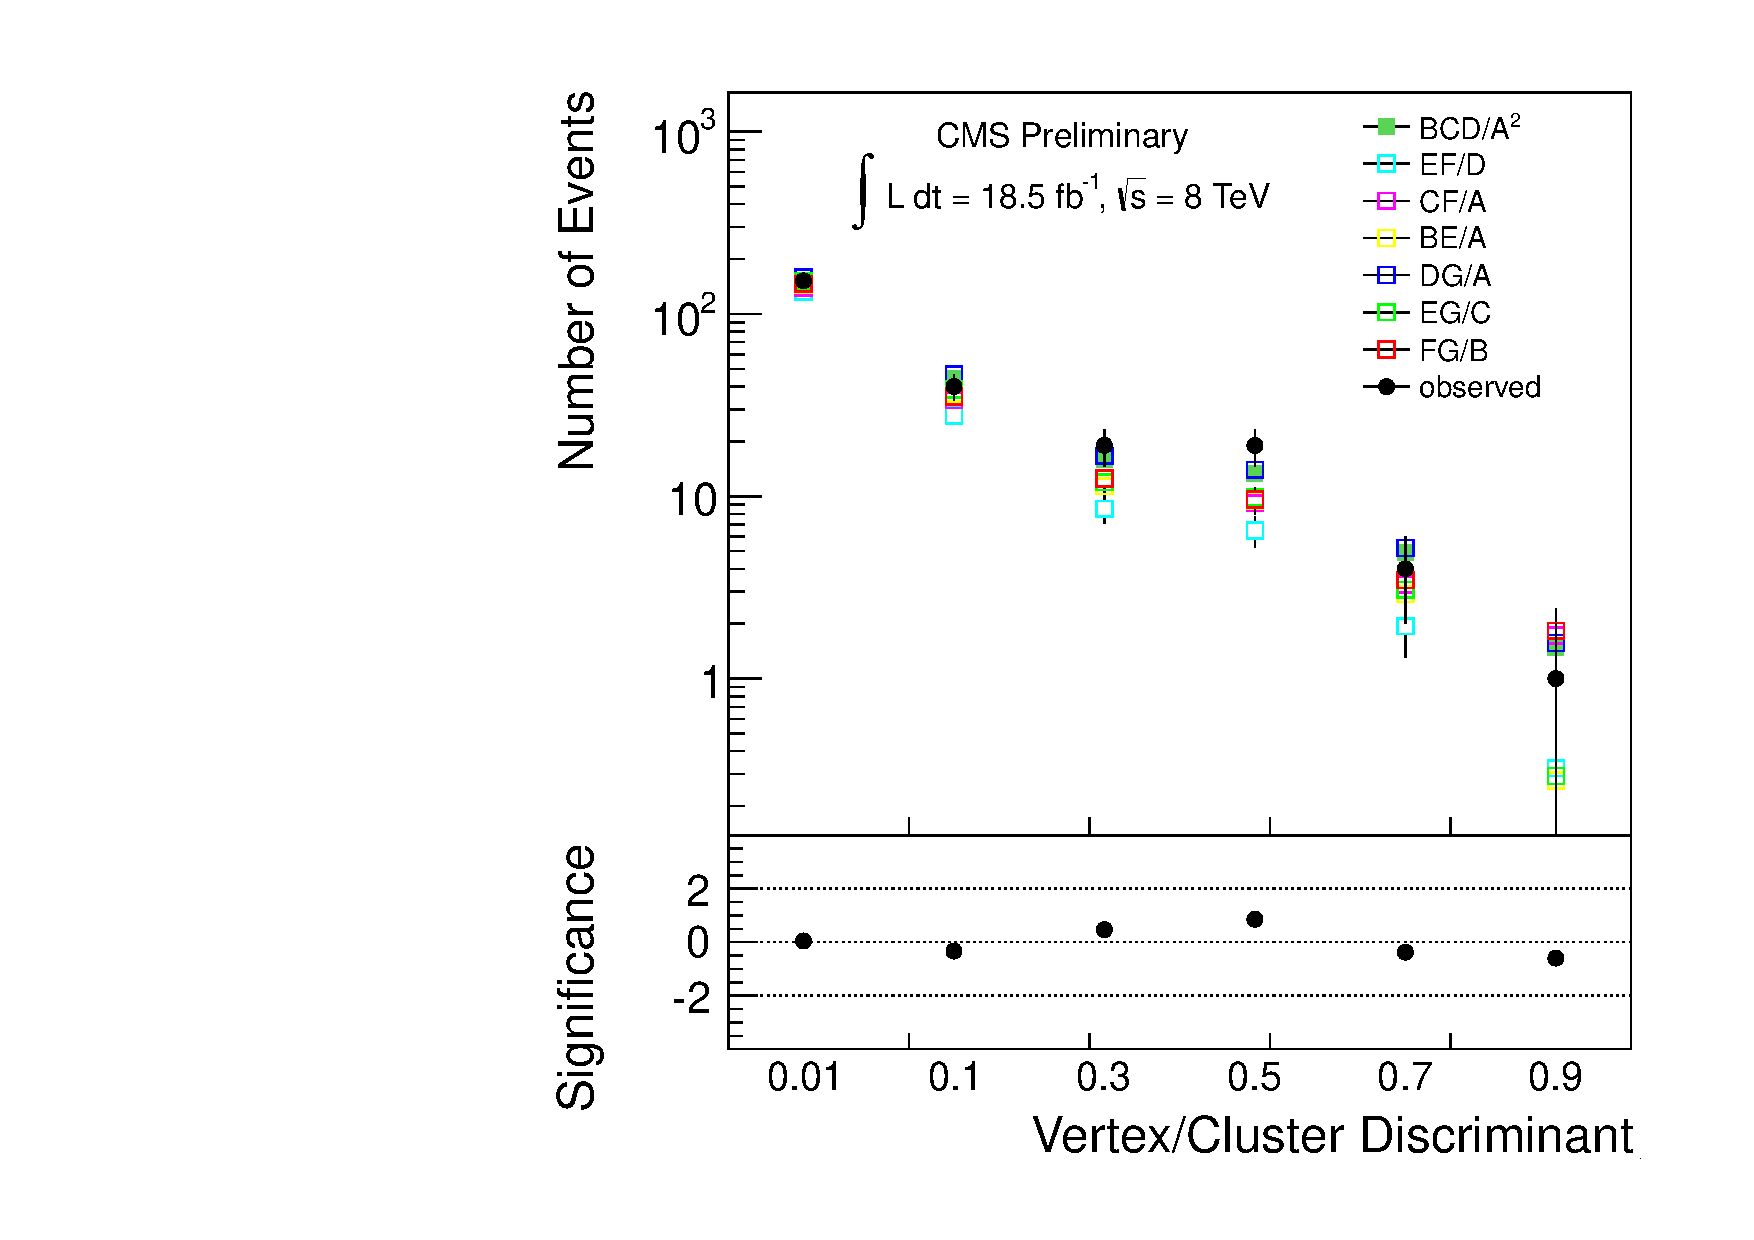
\includegraphics[width=0.495\textwidth]{plots/background/bkg_NMiss1.pdf}
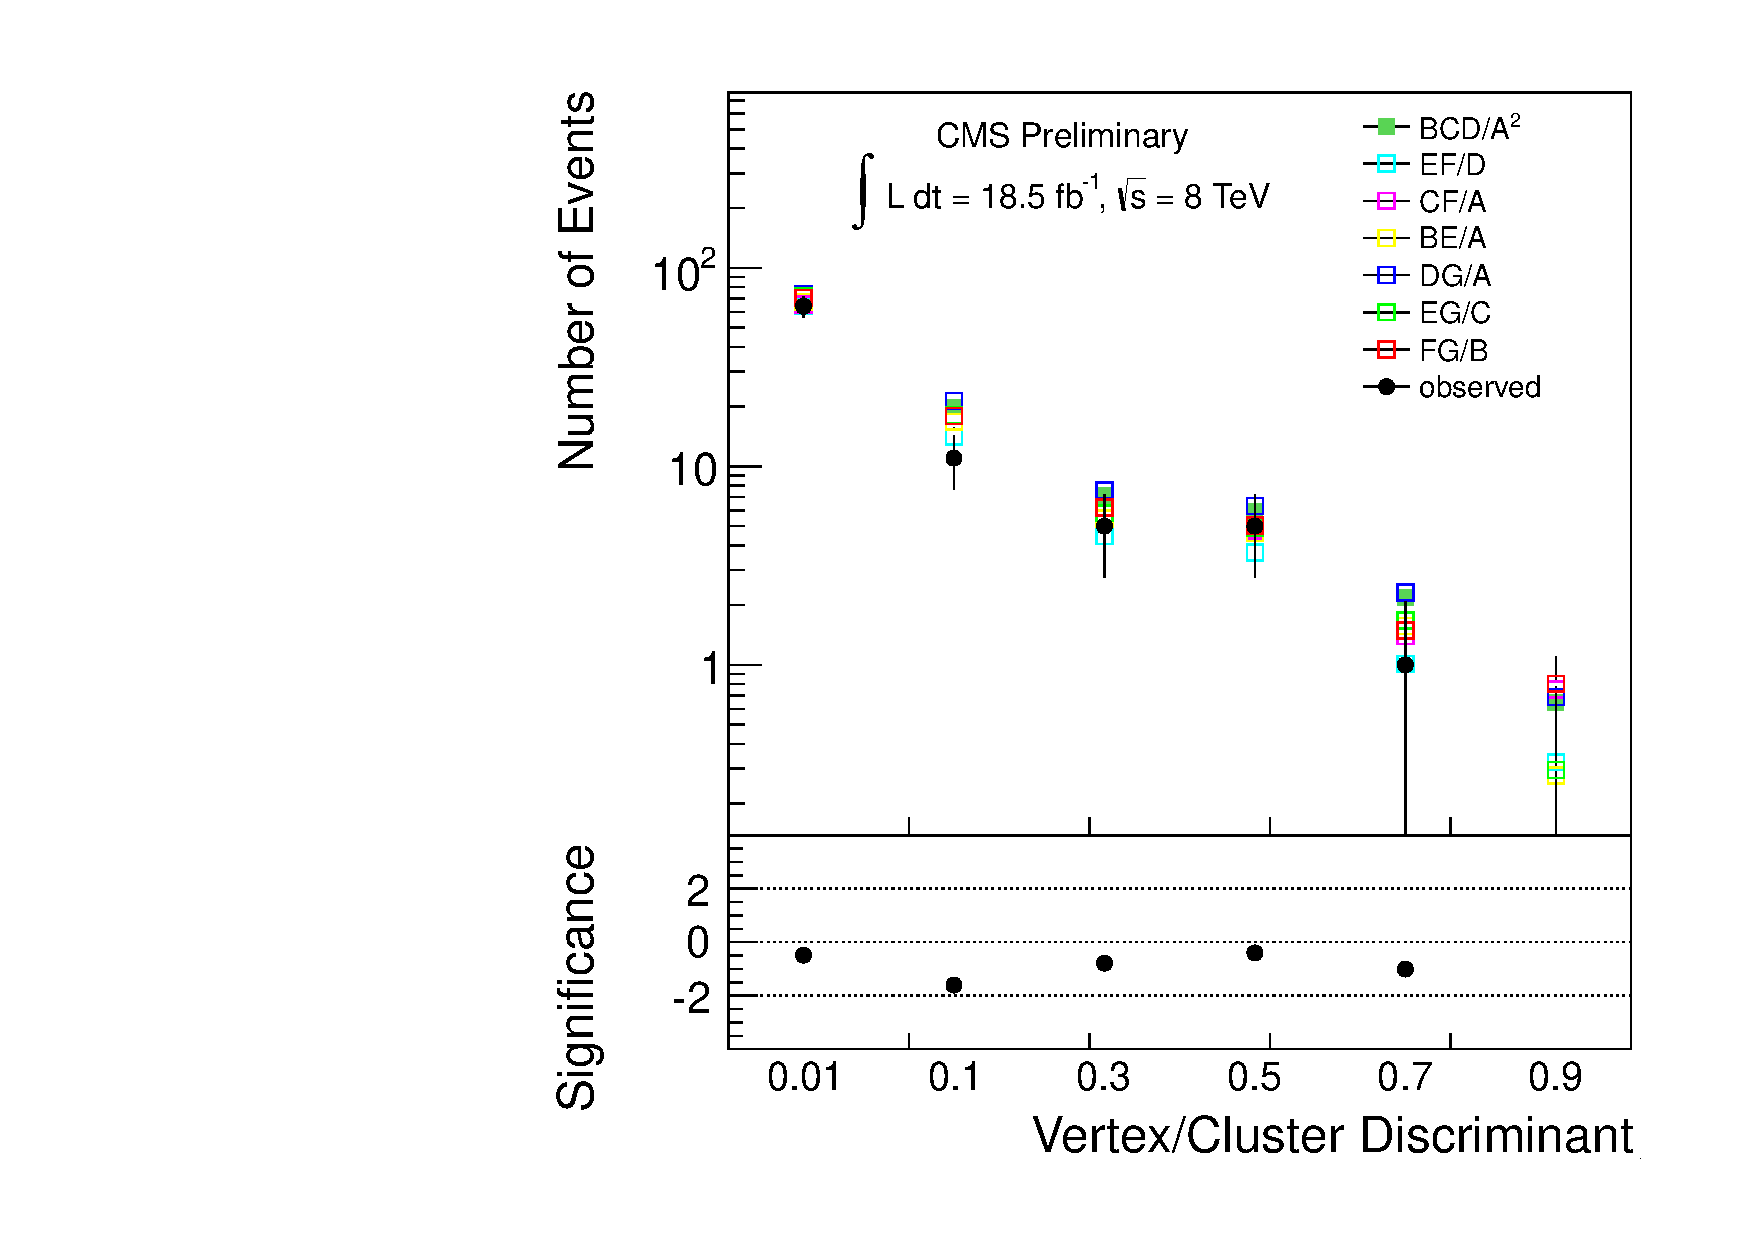
\includegraphics[width=0.495\textwidth]{plots/background/bkg_NMiss2.pdf}
\caption{Predicted and observed background levels in the data control region as a function of the vertex
discriminant selection criteria. The selection requires at most one prompt track and that the jet energy fraction carried by prompt tracks is
below 15\% and 9\% on the left and right plot, respectively.\label{fig:bkg_NMiss}}
\end{figure}

\section{Background estimate based on 10\% of the dataset}
\label{sec:partunblinding}

In order to check that there is no anomalous background present,
 we initially examined the data corresponding to only 10\% of all available 
data in the signal region.  
We select the data using one out of every ten luminosity sections, where a luminosity
section is a period of approximately 23 seconds of active data taking. This way of choosing the data is sensitive to possible problems that occur only for selected data taking periods, and also to effects that may arise from
correlations between consecutive events accepted by the trigger. A comparison of the data and predicted
background is presented in Fig. \ref{fig:10percent}. No anomalous background is observed in this sample,
however, the background predictions are small, thus limiting the statistical
power of the test.

\begin{figure}[htbp]
  \centering
  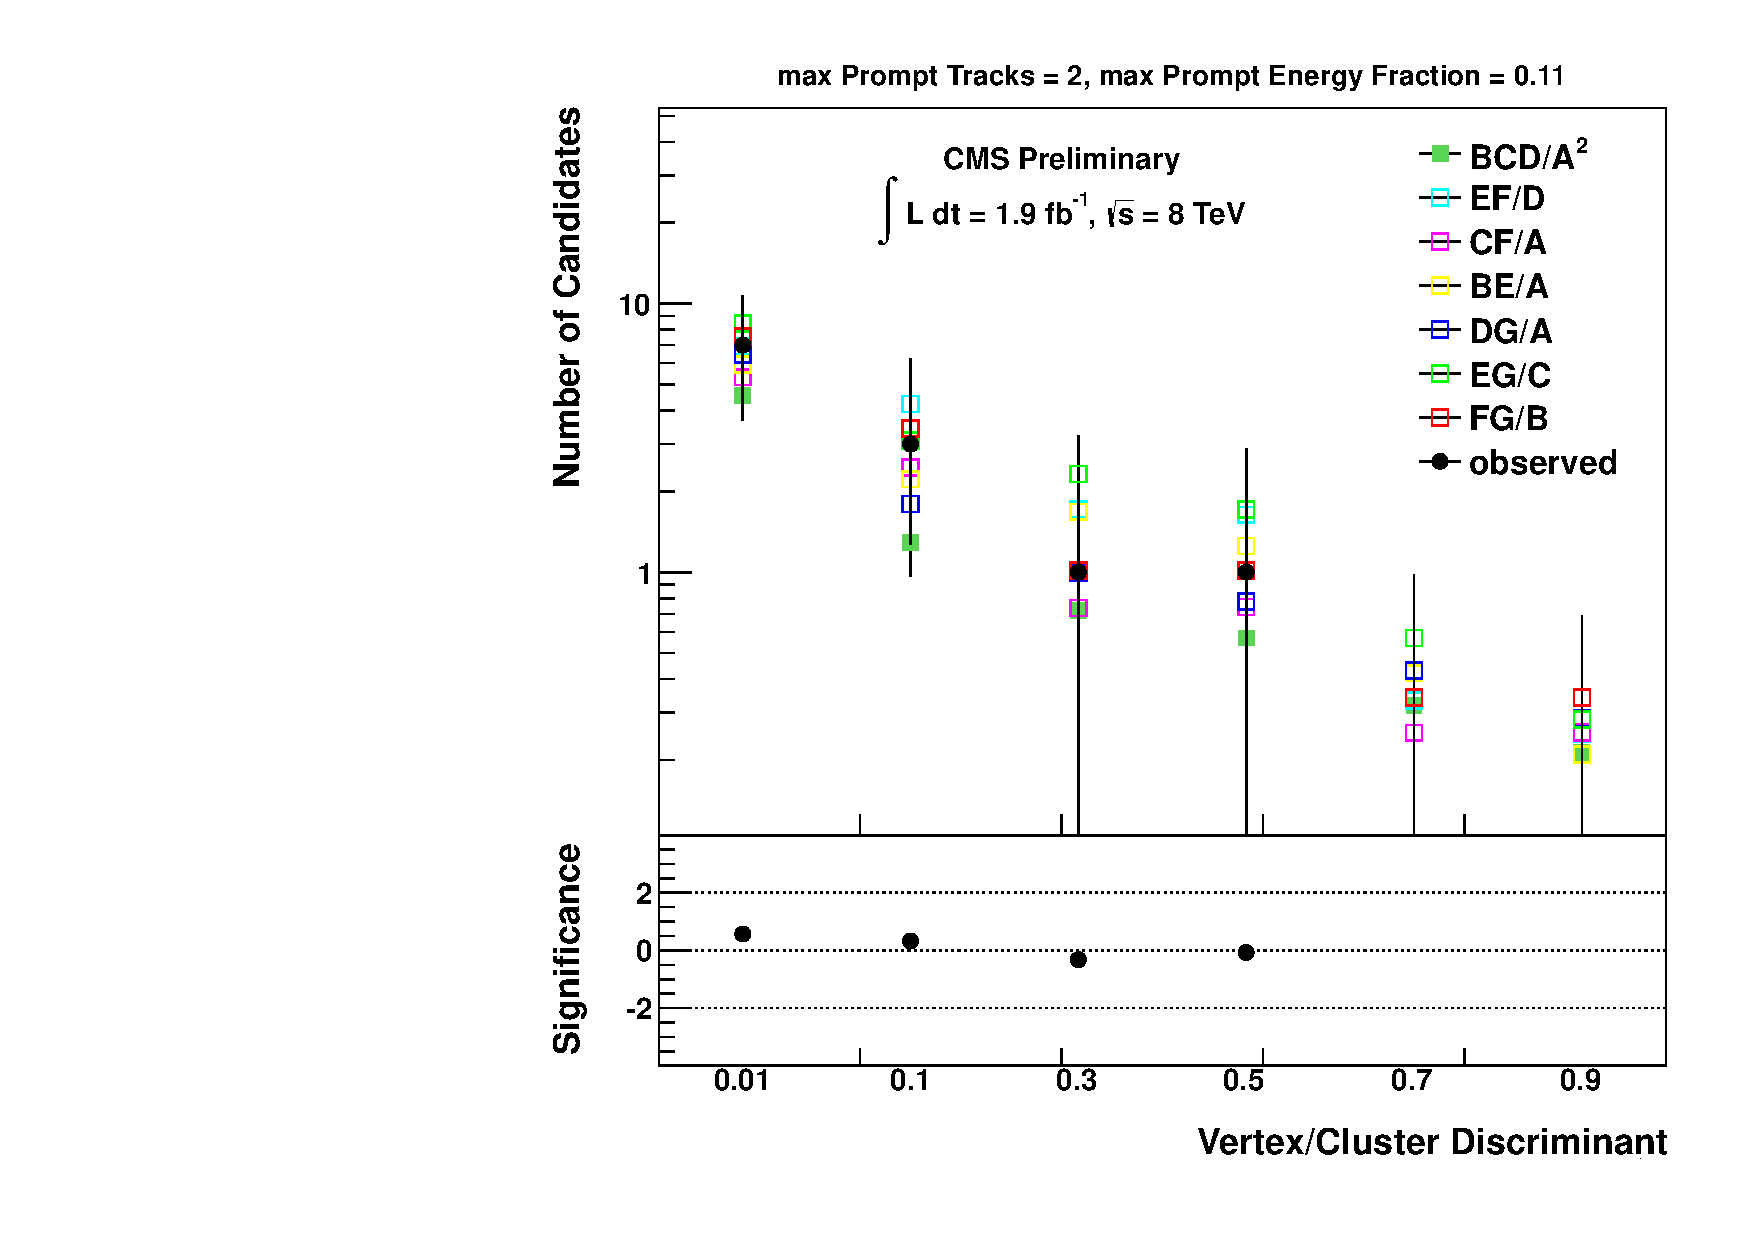
\includegraphics[width=0.495\textwidth]{plots/background/tenpercent1.pdf}
  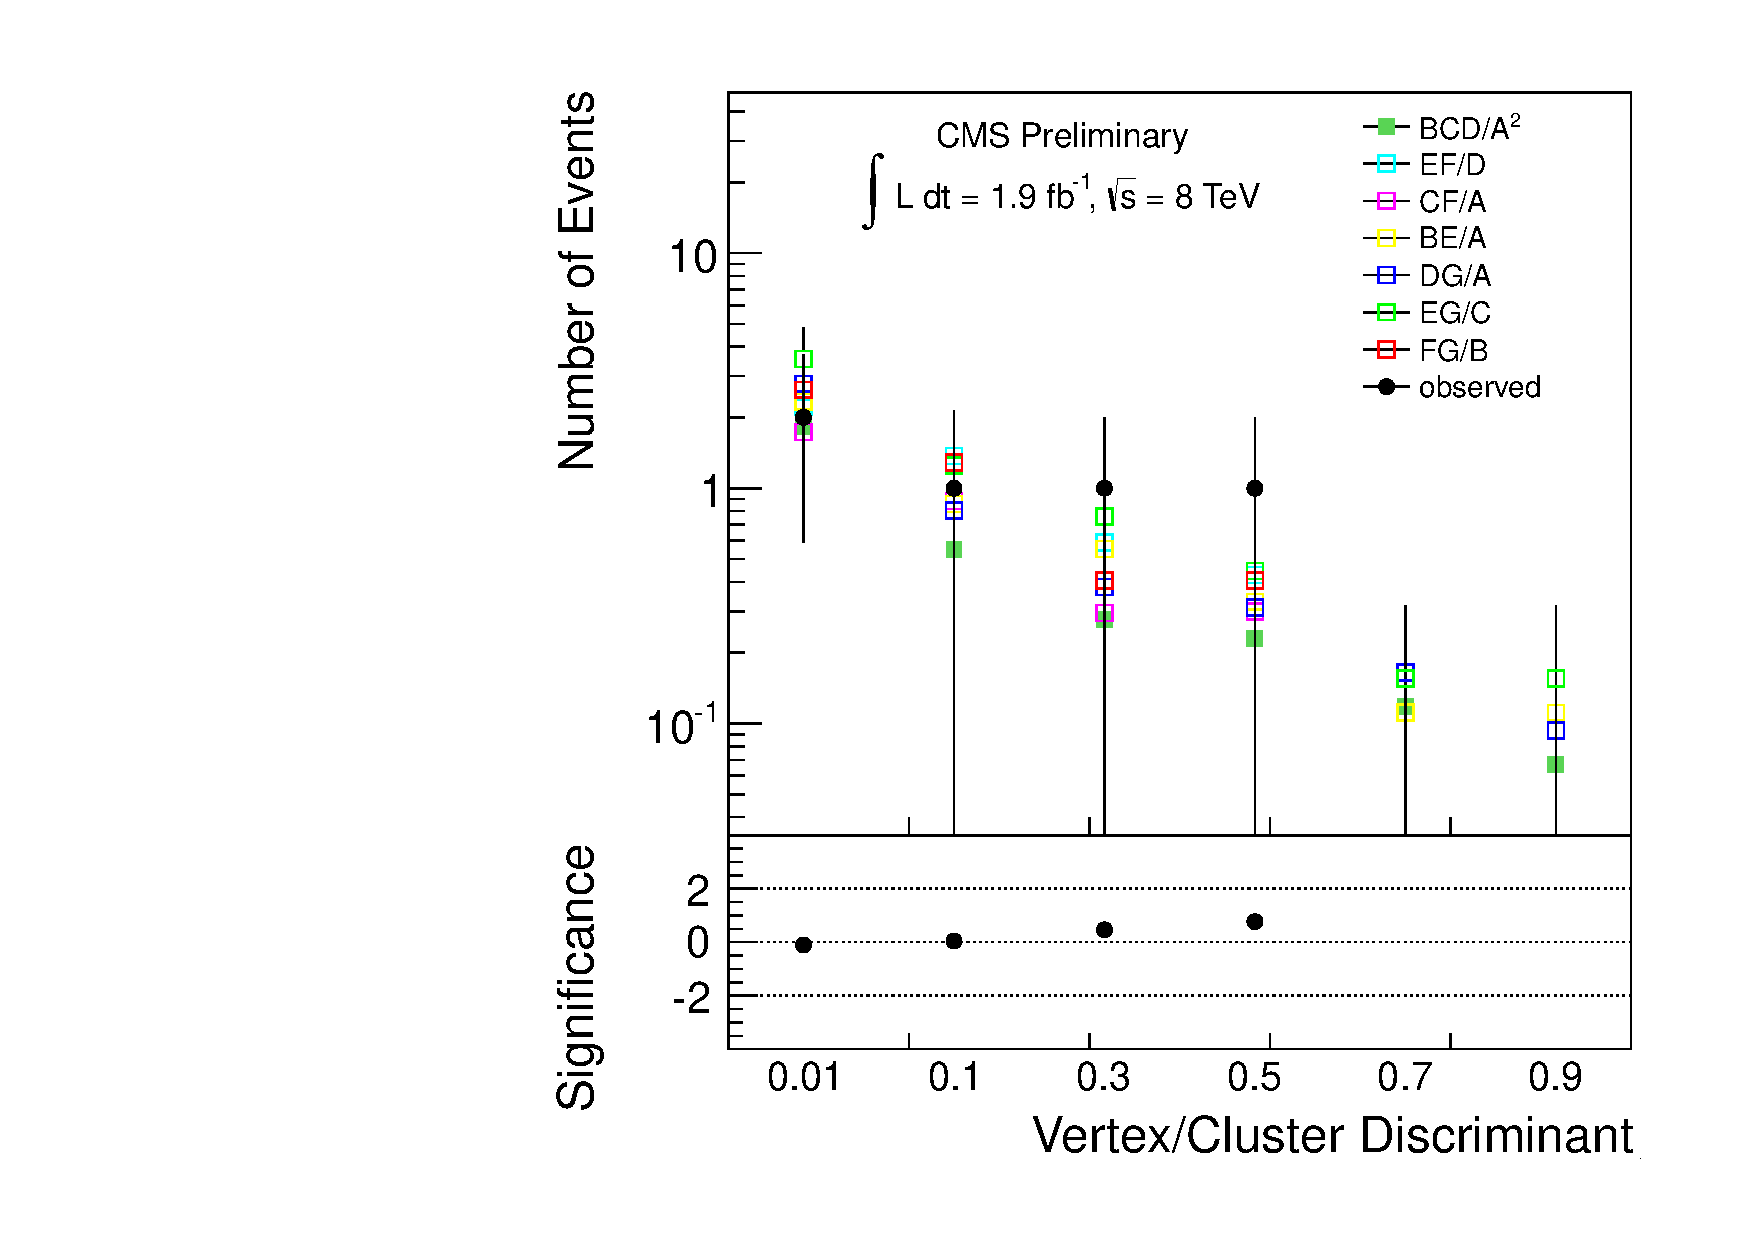
\includegraphics[width=0.495\textwidth]{plots/background/tenpercent2.pdf}
  \caption{Data and predicted background level in the 10\% data sample as a function of vertex discriminant
selection criteria. The selection requires at most 2 (left) or 1 (right) prompt tracks while the jet energy 
fraction carried by the prompt tracks is required to be less than 11\%. \label{fig:10percent}}
\end{figure}  


